\chapter{Objekterkennung mit der Top-down-Kamera}
\label{ch:objekterkennung}
% Verantwortlich: Person 1

Die Objekterkennung bestimmt aus einem Bild der Top-down-Kamera, wo das Bauteil im
Arbeitsbereich liegt und wie es gedreht ist. Das Ergebnis übergibt sie als
\texttt{ObjectPose} im Roboter-\ac{ks} an den Orchestrator (\cref{sec:schnittstellen}). Da
das Bauteil flach auf dem Tisch liegt, genügen dafür die Position $(x, y)$ in der Tischebene
und der Drehwinkel $\theta$ um die Hochachse; die Höhe ist durch die Tischhöhe festgelegt.

Die Verarbeitung ist als Kette von Einzelschritten aufgebaut (\cref{fig:m1-kette}). Sie
arbeitet ausschließlich auf dem übergebenen Bild und greift selbst nicht auf die Kamera zu.
Dadurch lässt sie sich mit gespeicherten Fotos genauso ausführen wie mit Live-Bildern
(\cref{sec:teststrategie}).

\begin{figure}[htbp]
  \centering
  \begin{tikzpicture}[
      box/.style={draw, rounded corners, align=center, minimum height=12mm, text width=38mm, font=\small},
      arr/.style={-{Stealth[length=2.2mm]}, thick},
      node distance=6mm and 8mm]
    \node[box] (a) {Kamerabild};
    \node[box, right=of a] (b) {Arbeitsbereich finden\\(ArUco-Marker)};
    \node[box, right=of b] (c) {Entzerrte Draufsicht\\(Homographie)};
    \node[box, below=of c] (d) {Bauteil segmentieren};
    \node[box, left=of d] (e) {Pose bestimmen\\(Schwerpunkt, Fase)};
    \node[box, left=of e] (f) {Transformation in\\das Roboter-\ac{ks}};
    \draw[arr] (a) -- (b);
    \draw[arr] (b) -- (c);
    \draw[arr] (c) -- (d);
    \draw[arr] (d) -- (e);
    \draw[arr] (e) -- (f);
  \end{tikzpicture}
  \caption{Verarbeitungskette der Objekterkennung}
  \label{fig:m1-kette}
\end{figure}

% ------------------------------------------------------------------------------
\section{Bildaufnahme und Kamerakalibrierung}
\label{sec:m1-kalibrierung}

Die Top-down-Kamera, eine Daheng VEN-161 mit $1440 \times 1080$~Pixeln und Global Shutter,
ist an einer Stange schräg über dem Arbeitsbereich montiert. Sie wird über das Software-Paket
des Herstellers angesprochen und über ihre Seriennummer ausgewählt, da am selben Rechner
eine baugleiche Handgelenkkamera für Modul~4 hängt. Dieselbe Kamera dient Modul~4 als
Szenenkamera; vor einer Fahrt von Modul~4 gibt die Objekterkennung sie frei und öffnet sie
beim nächsten Bild wieder (\cref{sec:m4-integration}). Die bisherigen Testbilder stammen von
einer Smartphone-Kamera aus derselben Perspektive.

Für reproduzierbare Ergebnisse soll die Belichtung fest eingestellt werden. Derzeit regelt
die Kamera Belichtung und Verstärkung noch automatisch. Eine Korrektur der
Linsenverzeichnung mit einer intrinsischen Kalibrierung nach Zhang (\cref{sec:kalibrierung})
ist vorgesehen, aber noch nicht umgesetzt. Die Verarbeitung arbeitet derzeit direkt auf dem
unkorrigierten Bild.

\todo[inline]{Montagehöhe ergänzen, feste Belichtung festlegen. Intrinsische Kalibrierung
durchführen und beschreiben, sofern sie umgesetzt wird.}

% ------------------------------------------------------------------------------
\section{Detektion des Arbeitsbereichs}
\label{sec:m1-arbeitsbereich}

Der Arbeitsbereich ist durch vier ArUco-Marker aus dem Wörterbuch \texttt{DICT\_4X4\_50}
mit den IDs~0 bis~3 festgelegt~\cite{garrido2014}. Die Marker sind auf Papier gedruckt und
auf die dunkle Platte geklebt; der weiße Rand um jeden Marker hebt dessen schwarze Kante vom
dunklen Untergrund ab. Ihre Mittelpunkte liegen \SI{400}{\milli\metre} auseinander und sind
im Arbeitsbereich-\ac{ks} in der Konfiguration hinterlegt (\cref{sec:koordinatensysteme}).

Die Marker werden mit dem ArUco-Detektor von OpenCV~\cite{bradski2000opencv} im
Graustufenbild gesucht; die Markerecken werden dabei subpixelgenau verfeinert. Aus den vier
Ecken jedes Markers wird dessen Mittelpunkt berechnet. Fehlt einer der vier Marker, bricht
die Verarbeitung mit einem Fehler ab, da die Lage des Arbeitsbereichs dann nicht eindeutig
bestimmt ist.

Die vier Markermittelpunkte im Bild und ihre bekannten Positionen im Arbeitsbereich bilden
vier Punktkorrespondenzen, aus denen eine Homographie zwischen Bildebene und Tischebene
berechnet wird (\cref{sec:aruco}). Mit ihr wird das Kamerabild in eine entzerrte Draufsicht
des Arbeitsbereichs umgerechnet. Sie zeigt das Quadrat von $330 \times 330$~\si{\milli\metre}
zwischen den Markern, sodass das helle Markerpapier außerhalb liegt. Die Draufsicht hat einen
festen Maßstab von \SI{2}{Pixel\per\milli\metre}; ein Pixel entspricht also
\SI{0,5}{\milli\metre} auf dem Tisch, und die Perspektive der schräg montierten Kamera ist
ausgeglichen. Alle weiteren Schritte arbeiten in dieser Draufsicht. \Cref{fig:m1-debug} zeigt
ein Kamerabild mit den erkannten Markern und die daraus berechnete Draufsicht.

Da die Marker in jedem Bild neu gefunden werden, ist ein Verschieben der Kamera für die
Objekterkennung unkritisch. Werden dagegen die Marker verschoben, müssen ihre Positionen neu
vermessen und die Kalibrierung zum Roboter wiederholt werden. Der Code enthält zusätzlich
einen Rückfall, der den Arbeitsbereich über die Innenkante eines weißen Rahmens findet; im
aktuellen Aufbau gibt es keinen solchen Rahmen mehr, und es werden nur die Marker verwendet.

% ------------------------------------------------------------------------------
\section{Segmentierung des Bauteils}
\label{sec:m1-segmentierung}

In der entzerrten Draufsicht muss das Bauteil vom Hintergrund getrennt werden. Die Platte
des Arbeitsbereichs ist dunkelgrau, das Bauteil dagegen heller oder farbiger. Die
Segmentierung prüft deshalb zwei Merkmale (\cref{sec:farbraeume}): die Helligkeit als
Hellwert $V$ des \ac{hsv}-Farbraums und die Buntheit als Chroma $C^*_{ab}$ des
CIELAB-Farbraums (\cref{eq:chroma}).

Anstelle fester Schwellwerte werden die Grenzen relativ zur Platte bestimmt. Da das Bauteil
nur einen kleinen Teil des Arbeitsbereichs bedeckt, beschreibt der Median von Hellwert und
Buntheit über die gesamte Draufsicht die Platte. Ein Pixel gilt als Bauteil, wenn sein
Hellwert um mehr als 50 oder seine Buntheit um mehr als 20 über dem Wert der Platte liegt.
Ändert sich das Raumlicht, verschieben sich Platte und Bauteil gemeinsam, und die Schwelle
wandert mit. Außerdem funktioniert die Segmentierung unabhängig von der Farbe des Bauteils,
solange es sich in Helligkeit oder Buntheit von der Platte abhebt. Ein globales
Schwellwertverfahren wie das nach Otsu (\cref{sec:bildverarbeitung}) wäre eine Alternative,
setzt aber ein deutlich zweigipfliges Histogramm voraus, das bei einem kleinen Bauteil auf
großer Fläche nicht gegeben ist.

In einer ersten Fassung wurde statt der Buntheit die Sättigung $S$ des \ac{hsv}-Farbraums
verwendet. Auf Testfotos des Aufbaus führte das zu Fehldetektionen. Auf der dunklen Platte
spiegelte sich in einer Ecke ein bläulicher Schimmer, und weil die Sättigung bei dunklen
Pixeln schon kleine Farbstiche stark gewichtet (\cref{sec:farbraeume}), erreichte dieser
Bereich Werte von 45 bis 58. Die Schwelle lag bei etwa 52 (Median der Platte plus 40), der
Reflex also teilweise darüber. In einem Bild war die so segmentierte Fläche größer als das
Bauteil und wurde an seiner Stelle ausgewählt; in einem anderen verschmolz sie mit dem
Bauteil und verfälschte Kontur und Orientierung. In der Buntheit sind die drei Flächen
dagegen klar getrennt (\cref{tab:m1-buntheit}): Die Schwelle (Platte plus 20, also 22 bis
23) liegt deutlich über dem Reflex und deutlich unter dem Bauteil. Mit ihr wird das Bauteil auf allen fünf
Testfotos korrekt segmentiert.

\begin{table}[htbp]
  \centering
  \caption{Sättigung und Buntheit auf den Testfotos (Median je Fläche, 8-Bit-Werte, fünf
  Fotos)}
  \label{tab:m1-buntheit}
  \begin{tabular}{@{}lcc@{}}
    \toprule
    Fläche & Sättigung $S$ & Buntheit $C^*_{ab}$ \\
    \midrule
    Platte              & 12--13 & 2--3 \\
    bläulicher Reflex   & 45--58 & 8--9 \\
    Bauteil (violett)   & 76--99 & 40--52 \\
    \bottomrule
  \end{tabular}
\end{table}

Die entstehende Binärmaske wird an einem schmalen Streifen von \SI{5}{\milli\metre} entlang
des Rands des Arbeitsbereichs beschnitten, damit Reste des Markerpapiers nicht als Bauteil
erkannt werden, und anschließend morphologisch bereinigt: Ein Öffnen
entfernt einzelne Störpixel, ein Schließen füllt kleine Lücken im Bauteil. Von den
gefundenen Konturen werden nur solche mit plausibler Fläche betrachtet; die größte davon
ist das Bauteil. Wird keine passende Kontur gefunden, meldet das Modul \enquote{kein Bauteil},
und der Orchestrator kehrt ohne Fehler in den Ruhezustand zurück.

% ------------------------------------------------------------------------------
\section{Bestimmung der Pose}
\label{sec:m1-pose}

Die Position des Bauteils ist der Flächenschwerpunkt der Kontur, der sich aus den
Bildmomenten nullter und erster Ordnung ergibt. Für die Orientierung wird das kleinste
umschließende Rechteck der Kontur bestimmt; seine lange Seite gibt die Längsachse des
Bauteils an.

Die Längsachse allein legt die Orientierung nur bis auf \ang{180} fest, da ein Quader in der
Draufsicht punktsymmetrisch ist. Eindeutig wird sie über die abgeschrägte Ecke des Bauteils:
An der Fase fehlt dem Bauteil eine Ecke, sodass genau eine Ecke des umschließenden Rechtecks
deutlich außerhalb der Kontur liegt. Für jede Rechteckecke wird der Abstand zur Kontur
berechnet. Liegt die am weitesten entfernte Ecke mehr als einen festen Anteil der
Bauteilbreite außerhalb, gilt die Fase als gefunden, und die Längsachse wird so ausgerichtet,
dass sie zur Fase zeigt. Der Winkel ist dann im Bereich \ang{0} bis \ang{360} eindeutig. Wird
keine Fase gefunden, wird der Winkel auf \ang{0} bis \ang{180} begrenzt und die Konfidenz der
Pose herabgesetzt. \Cref{fig:m1-pose} fasst das Vorgehen zusammen.

\begin{figure}[htbp]
  \centering
  \begin{tikzpicture}[font=\small, scale=1.1]
    \draw[fill=violet!20, thick] (0,0) -- (4,0) -- (4,1.1) -- (3.5,1.6) -- (0,1.6) -- cycle;
    \draw[dashed] (0,0) rectangle (4,1.6);
    \node[font=\scriptsize, anchor=east, align=right] at (-0.1,0.8) {umschließendes\\Rechteck $R$};
    \node[font=\scriptsize, anchor=north] at (2,0) {Kontur $K$};
    \node[font=\scriptsize, anchor=south] at (3.5,1.62) {Fase};
    \fill (4,1.6) circle (1.5pt) node[above right, inner sep=1pt] {$e_k$};
    \draw[{Stealth[length=1.5mm]}-{Stealth[length=1.5mm]}] (3.75,1.35) -- (4,1.6);
    \node[anchor=west, inner sep=1pt] at (4.05,1.25) {$d_k$};
    \fill (2,0.8) circle (1.5pt) node[below, inner sep=2pt] {$(u,v)$};
    \draw[pap arr] (2,0.8) -- (3.2,0.8) node[midway, above] {$\vec a$};
  \end{tikzpicture}

  \vspace{6mm}
  \begin{tikzpicture}[pap]
    \node[pap term] (start) {Kontur $K$ des Bauteils};
    \node[pap proc, below=of start] (sp) {Schwerpunkt $(u,v)$ aus den Bildmomenten};
    \node[pap proc, below=of sp] (rect) {Kleinstes umschließendes Rechteck $R$, Längsachse $\vec a$};
    \node[pap proc, below=of rect] (ecken) {Abstand jeder Ecke von $R$ zur Kontur, größter Abstand $d_k$ an Ecke $e_k$};
    \node[pap dec, below=of ecken] (fase) {$d_k > f \cdot b_R$\,?};
    \node[pap dec, below=of fase] (richt) {$\vec a$ zeigt\\zur Fase?};
    \node[pap proc=24mm, right=14mm of richt] (umk) {$\vec a$ umkehren};
    \node[pap proc, below=of richt] (w360) {$\theta$ aus $\vec a$ im Bereich $[\ang{0}, \ang{360}]$, Konfidenz $c = 1$};
    \node[pap proc=36mm, left=10mm of fase] (w180) {$\theta$ im Bereich $[\ang{0}, \ang{180}]$,\\Konfidenz $c = 0{,}5$};
    \node[pap term, below=of w360] (ende) {Pose $(u,v)$, $\theta$, $c$};
    \draw[pap arr] (start) -- (sp);
    \draw[pap arr] (sp) -- (rect);
    \draw[pap arr] (rect) -- (ecken);
    \draw[pap arr] (ecken) -- (fase);
    \draw[pap arr] (fase) -- node[pap lbl, right=1pt] {ja, Fase gefunden} (richt);
    \draw[pap arr] (fase) -- node[pap lbl] {nein} (w180);
    \draw[pap arr] (richt) -- node[pap lbl, right=1pt] {ja} (w360);
    \draw[pap arr] (richt) -- node[pap lbl] {nein} (umk);
    \draw[pap arr] (umk) |- (w360);
    \draw[pap arr] (w180) |- (ende);
    \draw[pap arr] (w360) -- (ende);
  \end{tikzpicture}
  \caption{Posenbestimmung mit Fasenerkennung. Oben: Kontur, umschließendes Rechteck und
  Abstand $d_k$ der Rechteckecke an der Fase. Unten: Ablauf; $b_R$ ist die Breite von $R$,
  $f$ ein fester Anteil.}
  \label{fig:m1-pose}
\end{figure}

% ------------------------------------------------------------------------------
\section{Transformation in das Roboterkoordinatensystem}
\label{sec:m1-transformation}

Schwerpunkt und Winkel liegen zunächst in Pixeln der Draufsicht vor. Wegen des festen
Maßstabs ergibt sich die Position im Arbeitsbereich-\ac{ks} durch Division durch den Maßstab.
Da die Bildzeilen nach unten, die $y$-Achse des Arbeitsbereichs aber nach oben zeigt, werden
dabei die $y$-Koordinate gespiegelt und das Vorzeichen des Winkels umgekehrt.

Anschließend wird die Pose mit der ebenen Starrkörpertransformation aus
\cref{sec:koordinatensysteme} in das Roboter-\ac{ks} überführt: Die Position wird gedreht und
verschoben, zum Winkel wird der Drehwinkel der Transformation addiert. Als Höhe wird die
Tischhöhe eingetragen. Das Ergebnis wird zusammen mit der Konfidenz und einem Debug-Bild als
\texttt{ObjectPose} zurückgegeben.

\begin{figure}[htbp]
  \centering
  \begin{minipage}[b]{0.56\textwidth}
    \centering
    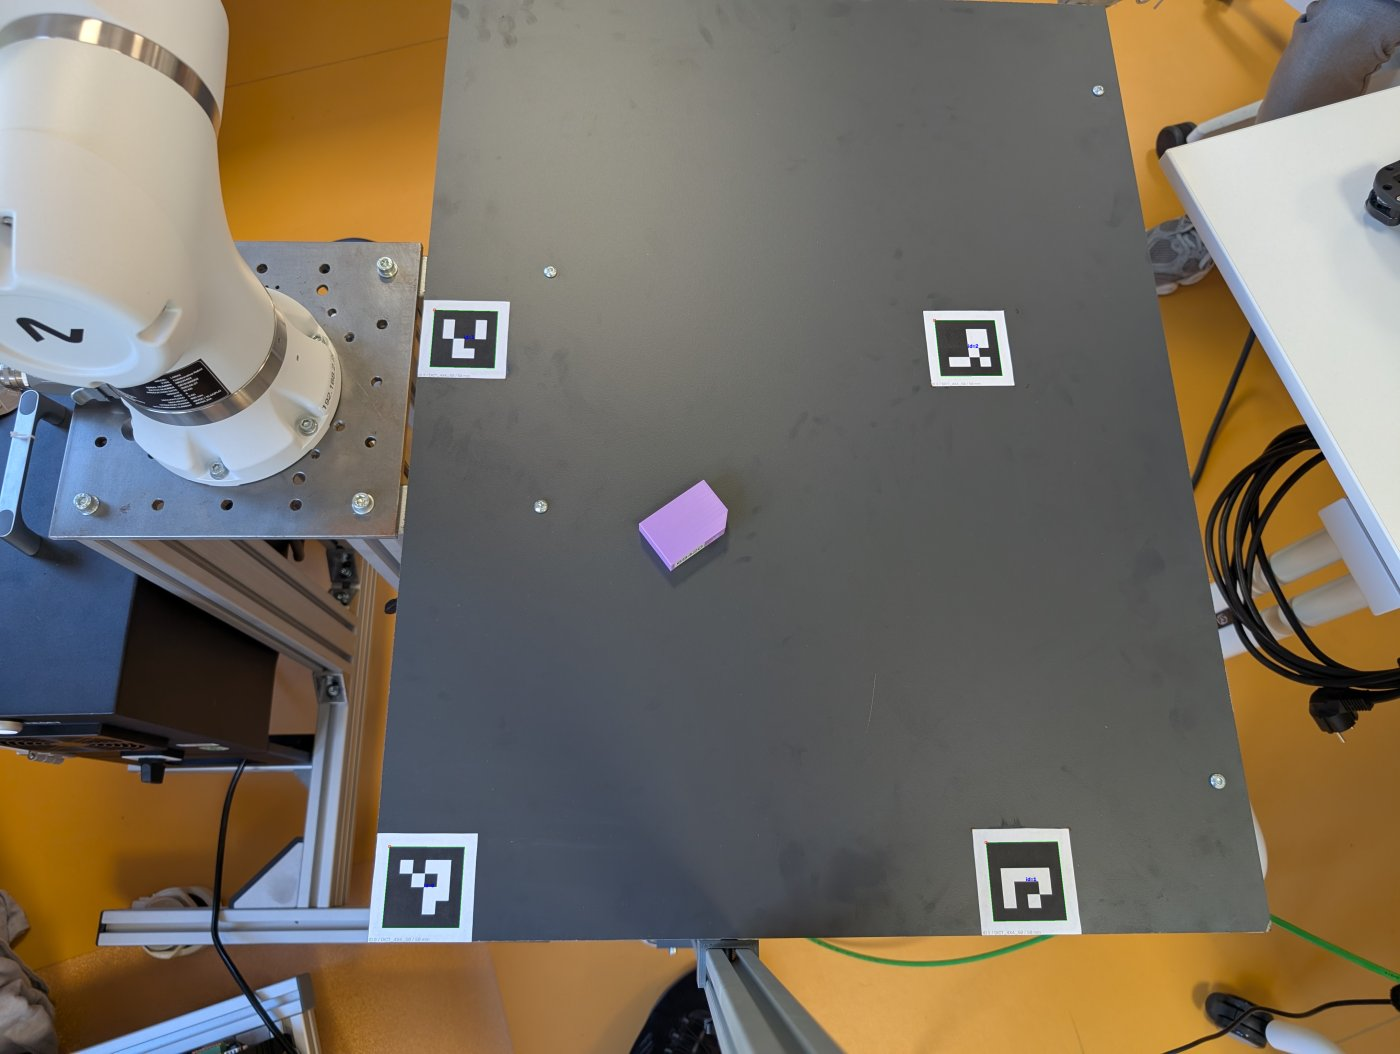
\includegraphics[width=\linewidth]{m1/m1_02_aruco_markers.jpg}
  \end{minipage}\hfill
  \begin{minipage}[b]{0.41\textwidth}
    \centering
    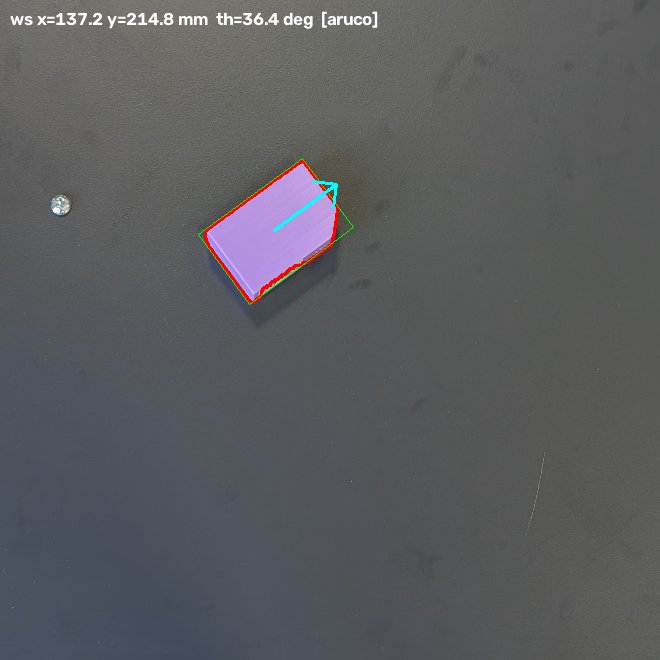
\includegraphics[width=\linewidth]{m1/m1_10_result.jpg}
  \end{minipage}
  \caption{Zwischenergebnisse der Objekterkennung an einem Testfoto: Kamerabild mit den vier
  erkannten Markern (links) und entzerrte Draufsicht des Arbeitsbereichs mit Kontur (rot),
  umschließendem Rechteck (grün) und Orientierung (Pfeil zur Fase); oben die Pose im
  Arbeitsbereich-\ac{ks} (rechts).}
  \label{fig:m1-debug}
\end{figure}

Die Transformation wird mit dem Roboter eingemessen (\cref{sec:koordinatensysteme}).

\subsection*{Parallaxe}

Die Homographie bildet die Tischebene maßstabsgetreu ab. Die Oberseite des Bauteils liegt
aber \SI{15}{\milli\metre} über dem Tisch, und bei der schräg blickenden Kamera sind zusätzlich
Seitenflächen sichtbar. Auf allen fünf Testfotos erscheint das Bauteil deshalb zu groß:
\numrange{64.5}{69.1}~\si{\milli\metre} $\times$ \numrange{43.3}{46.4}~\si{\milli\metre}
statt $60 \times 40$~\si{\milli\metre}, also \SIrange{8}{15}{\percent} mehr. Die Position ist
dabei stabil; drei Fotos derselben Lage weichen um höchstens \SI{0.4}{\milli\metre}
voneinander ab. Sie kann aber systematisch zur Bildmitte hin oder von ihr weg verschoben sein,
und zwar umso mehr, je weiter das Bauteil vom Punkt unter der Kamera entfernt liegt.

\todo[inline]{Parallaxe am Aufbau bewerten: Versatz im Zeigetest an Rand- und Mittelpositionen
notieren. Falls nötig korrigieren, z.\,B.\ die Oberseite statt der Tischebene entzerren.}

% ------------------------------------------------------------------------------
\section{Zwischenfazit}

Auf den Testfotos findet die Objekterkennung die Marker und das Bauteil zuverlässig und
bestimmt die Orientierung über die Fase eindeutig. Die gemessene Größe des Bauteils zeigt den
erwarteten Einfluss der Parallaxe. Wie stark er die Greifposition verschiebt, zeigt erst der
Zeigetest am Aufbau mit der endgültigen Kamera.

\todo[inline]{Nach den Versuchen ergänzen: Ergebnisse mit der Daheng-Kamera, Versatz im
Zeigetest, aufgetretene Probleme.}
